\documentclass[10pt]{article}
\usepackage{pgf,tikz,pgfplots}
\pgfplotsset{compat=1.15}
\usepackage{mathrsfs}
\usetikzlibrary{arrows}
\pagestyle{empty}
\begin{document}
\definecolor{xdxdff}{rgb}{0.49019607843137253,0.49019607843137253,1}
\definecolor{ududff}{rgb}{0.30196078431372547,0.30196078431372547,1}
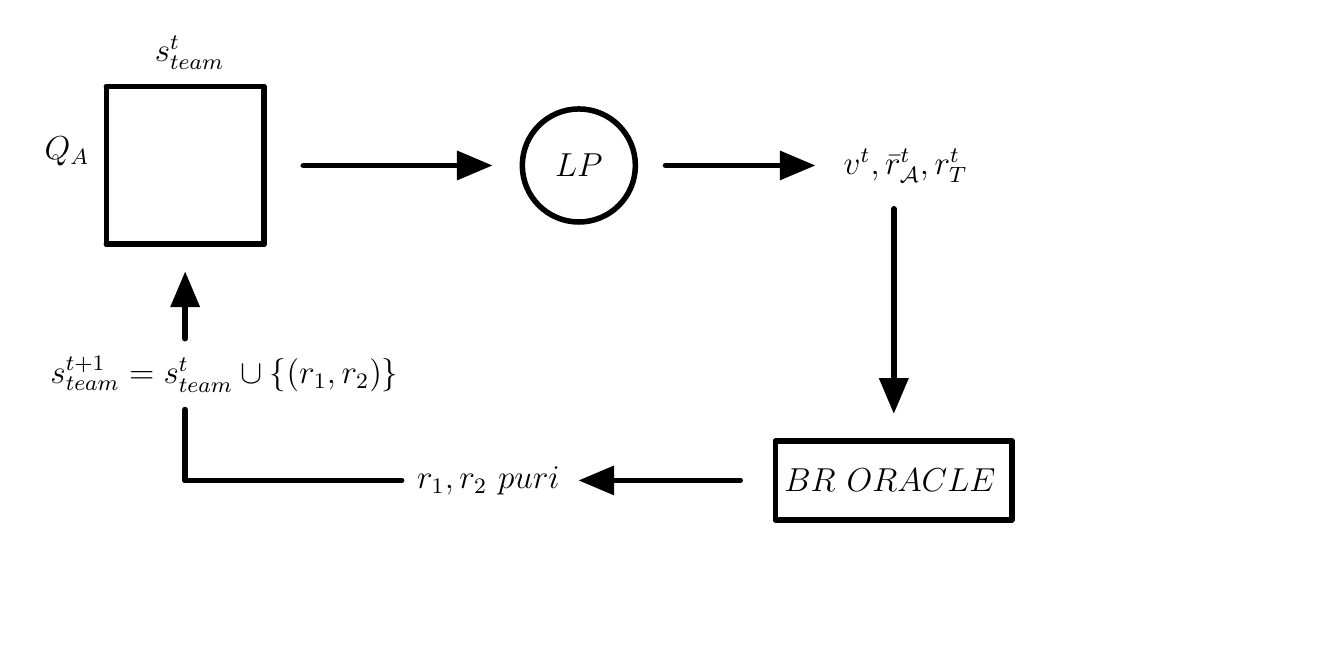
\begin{tikzpicture}[line cap=round,line join=round,>=triangle 45,x=1cm,y=1cm,scale=0.5,font=\large]
\clip(-14,-6) rectangle (18.5,9.5);
\draw [line width=2pt] (-12,8)-- (-12,4);
\draw [line width=2pt] (-12,4)-- (-8,4);
\draw [line width=2pt] (-8,4)-- (-8,8);
\draw [line width=2pt] (-8,8)-- (-12,8);
\draw [->,line width=2pt] (-7,6) -- (-2.2,6);
\draw [line width=2pt] (0,6) circle (1.4356939108665008cm);
\draw [->,line width=2pt] (2.2,6) -- (6,6);
\draw [->,line width=2pt] (8,4.9) -- (8,-0.3);
\draw [line width=2pt] (5,-1)-- (11,-1);
\draw [line width=2pt] (5,-3)-- (11,-3);
\draw [line width=2pt] (11,-3)-- (11,-1);
\draw [line width=2pt] (5,-1)-- (5,-3);
\draw [->,line width=2pt] (4.1,-2) -- (0,-2);
\draw [line width=2pt] (-4.5,-2)-- (-10,-2);
\draw [->,line width=2pt] (-10,1.6) -- (-10,3.3);
\draw [line width=2pt] (-10,-2) -- (-10,-0.2);
\begin{scriptsize}
\draw[color=black] (-13,6.357560057226035) node {$Q_A$};
\draw[color=black] (-9.887857943911982,8.86941565160432) node {$s_{team}^t$};
\draw[color=black] (0,6) node {$LP$};
\draw[color=black] (8.3,6) node {$v^t,\bar{r}_{\mathcal{A}}^t,r_T^t$};
\draw[color=black] (7.9,-2) node {$BR ~ ORACLE$};
\draw[color=black] (-2.3,-2) node {$r_1,r_2 ~ puri$};
\draw[color=black] (-9,0.7) node {$s_{team}^{t+1}=s_{team}^{t} \cup \{(r_1,r_2)\}$};
\end{scriptsize}
\end{tikzpicture}




\definecolor{ccqqqq}{rgb}{0.8,0,0}
\begin{tikzpicture}[line cap=round,line join=round,>=triangle 45,x=1cm,y=1cm,scale=0.6,font=\large]
\clip(-16.224120596005072,-6.164707365141574) rectangle (12.698861870761316,9.591515253324562);
\draw [line width=2pt] (-12,6)-- (-12,4);
\draw [line width=2pt] (-12,4)-- (-4,4);
\draw [line width=2pt] (-12,6)-- (-4,6);
\draw [line width=2pt] (-4,6)-- (-4,4);
\draw [->,line width=2pt] (-3,5) -- (3,5);
\draw [->,line width=2pt] (5,4) -- (5,1);
\draw [->,line width=2pt] (3,0) -- (-3,0);
\draw [line width=2pt] (-4,1)-- (-4,-1);
\draw [line width=2pt] (-12,1)-- (-12,-1);
\draw [line width=2pt] (-12,-1)-- (-4,-1);
\draw [line width=2pt] (-12,1)-- (-4,1);
\draw [->,line width=2pt] (-8,1.5) -- (-8,3.5);
\draw [->,line width=2pt,color=ccqqqq] (-8,-2) -- (-8,-4);
\begin{scriptsize}
\draw[color=black] (-8,5) node {$\bar{r}_1 ~ generator$};
\draw[color=black] (5,5) node {$\bar{r}_1,\bar{r}_{\mathcal{A}}$};
\draw[color=black] (5,0) node {$u_{\bar{\bm{\pi}}_1,\bar{\bm{\pi}}_{\mathcal{A}}}$};
\draw[color=black] (-8,0) node {$BR~player~2$};
\draw[color=black] (-7.3,2.2) node {$R$};
\draw[color=ccqqqq] (-8,-5) node {$(r_1^*,r_2^*)$};
\end{scriptsize}
\end{tikzpicture}

\end{document}